%% $RCSfile: proj_report_outline.tex,v $
%% $Revision: 1.3 $
%% $Date: 2016/06/10 03:41:54 $
%% $Author: kevin $

\documentclass[11pt
              , a4paper
              , twoside
              , openright
              ]{report}


\usepackage{float} % lets you have non-floating floats

\usepackage{url} % for typesetting urls

\usepackage[toc,page]{appendix}
\usepackage{pdfpages}
\usepackage{fancyhdr}

\graphicspath{ {images/} }


%
%  We don't want figures to float so we define
%
\newfloat{fig}{thp}{lof}[chapter]
\floatname{fig}{Figure}

%% These are standard LaTeX definitions for the document
%%                            
\title{FACT - A Micro Learning Management Tool}
\author{Callum Gill}

%% This file can be used for creating a wide range of reports
%%  across various Schools
%%
%% Set up some things, mostly for the front page, for your specific document
%
% Current options are:
% [ecs|msor|sms]          Which school you are in.
%                         (msor option retained for reproducing old data)
% [bschonscomp|mcompsci]  Which degree you are doing
%                          You can also specify any other degree by name
%                          (see below)
% [font|image]            Use a font or an image for the VUW logo
%                          The font option will only work on ECS systems
%
\usepackage[image,ecs,mcompsci]{vuwproject}

% You should specifiy your supervisor here with
\supervisor{Alex Potanin}
% use \supervisors if there is more than one supervisor

% Unless you've used the bschonscomp or mcompsci
%  options above use
\otherdegree{Bachelor of Engineering with Honours}
% here to specify degree

% Comment this out if you want the date printed.
\date{}

\begin{document}

% Make the page numbering roman, until after the contents, etc.
\frontmatter

%%%%%%%%%%%%%%%%%%%%%%%%%%%%%%%%%%%%%%%%%%%%%%%%%%%%%%%

%%%%%%%%%%%%%%%%%%%%%%%%%%%%%%%%%%%%%%%%%%%%%%%%%%%%%%%

\begin{abstract}

A short description of the project goes here.

\end{abstract}

%%%%%%%%%%%%%%%%%%%%%%%%%%%%%%%%%%%%%%%%%%%%%%%%%%%%%%%

\maketitle

\chapter*{Acknowledgments}\label{C:ack} 
Any acknowledgments should go 
in here, between the title page and the table of contents.  The 
acknowledgments do not form a proper chapter, and so don't get a 
number or appear in the table of contents.

\tableofcontents

% we want a list of the figures we defined
\listof{fig}{Figures}

%%%%%%%%%%%%%%%%%%%%%%%%%%%%%%%%%%%%%%%%%%%%%%%%%%%%%%%

\mainmatter

%%%%%%%%%%%%%%%%%%%%%%%%%%%%%%%%%%%%%%%%%%%%%%%%%%%%%%%

% individual chapters included here
\chapter{Introduction}\label{C:intro}
This project aims to develop a product that solves the problem of presenting essential information to employees in a concise, easy to read and measurable way. This project was suggested as further development of a proof of concept that HAUNT, a small web development company suggested. HAUNT acted as an industry supervisor for this project development as well as product owner. The product aims to be a micro learning management system that reduces a lot of the overhead of HR around keeping employees informed about procedures and policies within a company. This report will cover the motivations behind this product, the development and implementation of the product, engineering choices involved and the evaluation of the product with expert feedback. As this product will be developed in a start-up environment this report will also cover the challenges that software development faces in these environments.

\section{Haunt}
HAUNT is a start up company that develops and maintains various websites. As they are a new company they have recently gone through the human resource management of hiring new employees and informing them of company policies, health and safety and information on the company and relevant technology. They identified the potential need for a system to easily convey and manage this information quickly and efficiently.

\section{Start-ups}
Many start ups fail or find it difficult to develop their own products efficiently this can be effected by multiple factors, they potentially lack experience in small product development or within the target market, the market isn’t large enough to sustain the product, they have no users to establish feedback and/or validate ideas. This project will attempt to implement a process model that is effective when working in a start up environment without an established user base.

\subsection{Difficulties within start-ups}
As stated before start up companies often fail within their infancy. They can fail due to failures in ”execution of sales, marketing and delivery” [3] of their products. We will focus on process for product development and delivery that would be effective in a start up environment. The problematic issues of start ups and small companies when it comes to product deliveries include:

\begin{itemize}
\item Developers are inexperienced
\item Product over fitting (product may be highly customized or targeted towards a certain user)
\item Small/non-existent user base
\end{itemize}

These issues can be mitigated by proper planning and a well versed development process model. We will explore why some of these become issues.

\subsection{Developers are inexperienced}
This may or may not be the case in start ups as many developers come from or have some experience in product delivery management. However when dealing with smaller companies and their own products they often fall into methods and processes that harm the development of the product. This can be easily solved by ensuring the head developer of a product is highly experienced and won’t neglect important non-coding issues such as architecture, design, testing and documentation. Having a technical lead whom is experienced helps the potentially less experienced colleagues keep on track when it comes to the non-coding standards.

\subsection{Product over fitting}
When a start up company is developing a small product they have a tendency to over fit their product to a certain user. This is because they have such a small or non existent user base they only have a few sources of feedback and if they over value this feedback they may end up with a product that isn’t really suited to other users. To solve this, developers and project managers need to take any feedback that they gather from their users or themselves if they are the only test cases and make sure that it aligns with the goals of the product. Often less, better designed features are more effective than a product full of many half completed features.

\subsection{Small/non-existent user base}
Start up companies often have a limited user base or none at all. The problem with this is it increases the difficulty of gathering requirements from users and the feedback that you do receive is often from the same source. Therefore it can contribute to the over fitting problem. This is the type of environment that this project will be focusing on, the development of a product in an environment with little to no established user base.

\subsection{Summary}
To try and mitigate these issues we needed to implement a development model that helps reduce these potential problems. We needed to ensure that we have a proper authority structure, we have a process for requirement gathering and that we focus on the products goals to try and reduce over fitting to a certain user, including Haunt.

\section{Problem and Motivation}
The problem identified by HAUNT was the lack of a lightweight system that could be easily updated, inform users of their relevant information and present the required information in a non intrusive and intuitive manner that portrayed the important information without being overbearing. While there are some current solutions for information management systems and learning management systems, neither solve the issue of being too information dense and hard to update appropriately for a small HR team.

The main problem can be split up into two issues, the display, organization and management of the information and the notifications to the user along with displaying user relevant information. These issues is what this product tries to solve.

\section{Available Solutions}
As stated previously, there are two potential types of product that partially solve the issues identified. These are learning management tools (LMS) and knowledge management systems (KMS). However these solutions are only partial solutions to the problem and are aimed at solving different but similar issues. This report explores these current solutions and identifies the components that work well and the areas that they are lacking.

\section{Solution}
The suggested solution is a micro learning management system which address the need for a more lightweight knowledge management system that is easy to update and organize. It solves some of the issues that the current solutions involve such as user targeted information, a more lightweight display of information and an ease of updating information and informing users.
\chapter{Background}
This chapter explores current solutions that a company could use for managing company information and policies and the informing of staff. The main aspects that we will be exploring are the organization of information, the presentation and navigation of this information for users and the ease of updating this information and informing users of these changes that they may need to be made aware of. We will explore two main solution types, knowledge management systems and learning management systems.

\section{Knowledge Management Systems}
Knowledge management systems main goal is to provide effective and efficient knowledge management. This includes the need to archive information and provide an interface for easily retrieving and display this information. They often take the form of collaboratively driven systems known as Wikis. Wikis provide an environment for conversational knowledge to be created and iteratively improved in an ad-hoc manor and `combine the best elements of earlier conversational knowledge management technologies, while avoiding many of their disadvantages' \cite{maier2011knowledge, leuf2001wiki}.

\subsection{Wikis}
A Wiki refers to is a set of linked web pages that are created by incremental changes applied by a group of collaborating users and the software that is used to manage the pages and information. The key characteristics of a wiki are:

\begin{itemize}
\item It enables web documents to be authored collectively.
\item It uses a simple markup scheme (usually a simplified version of HTML, although HTML is frequently permitted).
\item Wiki content is not reviewed by any editor or coordinating body prior to its publication.
\item New web pages are created when users create a hyperlink that points nowhere.
\end{itemize}

From these characteristics you can see that Wikis are a collaborative system that relies on group contribution to remain up to date and the creation of new content. This creates a large knowledge base that can be updated easily and frequently with  an active community. However because of the lack of moderation outside of community amendments, some of the published knowledge can be incorrect. This is contrary to what is required within a company for documents such as policies and other content that requires an approval process.When Wikis have been used as company KMS they often exhibit multiple issues these have been identified as \cite{kiniti2013wikis}:

\begin{itemize}
\item Lack of a clear purpose for the wiki. Wikis are often created by individuals or small team and are then adopted by other teams or individuals.
\item Usability. These issues range from poor hosting infrastructure, user knowledge of syntax, duplicated data and validity of data.
\item Integrating the wiki into established work practices. 
\item Role of management. Usage of Wikis is gated by management involvement, encouragement, training and rewarding wiki users all contribute to a more successful wiki.
\item Social issues. A critical mass of users is required for a successful wiki.
\item Organizational Culture. Users are required to be open to sharing knowledge.
\end{itemize}

\section{Learning Management Systems}
LMS serve three main purposes, to manage users (both learners and facilitators), track online learning and progress and keep records of activity. LMS are often split into two sub categories, corporate or education, each focusing on a different learning environment. These share many characteristics and there is often overlap between the categories. Common features of a LMS include \cite{mcintosh2014vendors}:

\begin{itemize}
\item Online Courses
\item Classroom management
\item Communication and collaboration tools
\item Content management and development tools
\item Assessment and testing
\item Reporting
\end{itemize}

Each LMS offers its own suite of functionality, because of this they can fit a multitude of roles in numerous different environments. But the end goal of most them is to create and manage a collaborative online or blended learning environment. One of the most popular LMS's that many others are based on or extend is Moodle.

\subsection{Moodle}
Moodle is an open-source free LMS that is distributed under the GNU public license. Moodle is overall designed to promote community-oriented learning methodology, involving collaborative activities and active participation from its users. This is aimed at creating an online learning community. Moodle includes a multitude of community features such as, forums, blogs, announcements and wikis. It also includes learning management and tracking features such as tests and quizzes, assignments, report, student profiles and activity tracking \cite{mcintosh2014vendors, muhsen2013moodle}. However because of the multitude of features, like many LMS it requires training to use and manage effectively. Also for some of it applications it is over engineered and many of its features go unused or used improperly/poorly. This is a factor with broad LMS systems, because they target a broad range of applications, they lack the clarity of how to best use their features or they some of the features are adapted in incorrect or inefficient ways.

\section{Summary}
There are many KMS and LMS systems that can be used for managing and teaching information for employees. However, neither of them have them as their primary use. KMS are used to store and retrieve this information but have no designated tracking of learning or directed learning environment. While LMS are over engineered towards learning, are focused on a collaborative learning experience and the testing or validation of the users learning rather than a source for easy to navigate information that is targeted towards the user automatically.

\chapter{FACT}

\section{Goal}
The aim of FACT is to be a solution for provide a system for use within a corporate setting that presents required information and company policies to the employees in small, easy to digest chunks. This is to solve the problem of informing employees of information and being able to check if employees have actually read the information as well as providing a platform for reference material or training. What Haunt found when they were going through the early stages of their company development process was that there was a lack of effective and efficient applications that are effective at informing employees of essential information in a corporate environment, such as health and safety and other company policies. They established that there was a market for a solution that addresses this need for a lightweight application that can be used as an on boarding education tool as well as continued education of company policies. The solution would also notify employees of changes to policies that are relevant to them and allow a manager to ensure that their staff were up to date with company policies. The product should also be scalable to contain enough information that is easily navigable that it could replace or be used in conjunction with other knowledge management systems such as company wikis.

\section{FACT - The Product}
FACT is a micro-learning management tool that offers the ability to manage information on company policies, procedure and other employee on boarding necessities. The final product will also keep track of what users have read, notify them of any changes to the information that needs to be read and allows an administrator to monitor user participation. This information will be organized into decks that would be similar to courses in a more fully fledged learning management system. These decks will be the topics that a user could have assigned to them as required for their role. Decks will be filled with chunks of information called cards and/or facts. These will have a word limit on them to promote smaller chunks of information so they users are more likely to read them.

\section{Features}
\subsection{Users and Organisations}
Organisations will be the account that a user will be registered under. Users under the same organisations will be able to access  the same resources such as decks, cards and tags. The users will be rather simple entities that can be linked to decks through tags and able to be assigned a role for their access rights. A user will need to keep track of the completed cards and when/what version of each card was completed.

\subsection{Decks, Cards and Tags}
Cards would only contain snippets of information that could be easily digestible and mark off as understood. Cards should present the information in a way that the user can easily view all the information and tick them off once they are understood. Cards could also have the ability to show media such as images or video. The editing and restrictions for the cards should promote the idea of this bite sized information. The aim of a card or fact is to convey information that is a self sufficient piece of information, further detailed information could be linked to provide a more thorough overview (See \ref{fig:pitchdecks}).

\begin{figure}[h]
\label{pitchdecks}
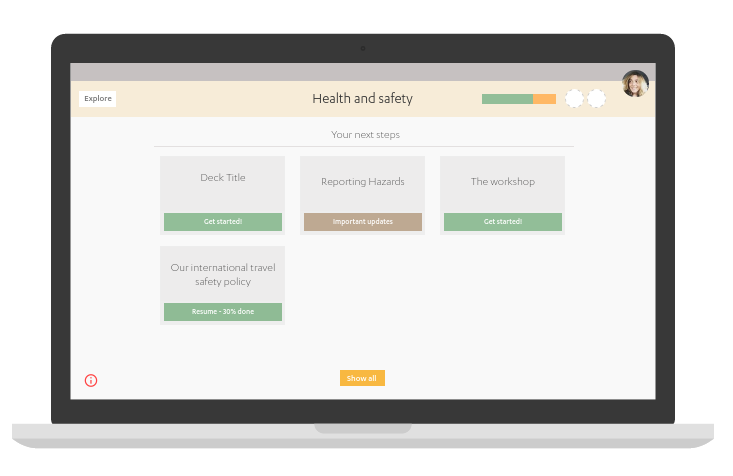
\includegraphics[width=\textwidth]{pitch-decks01}
\caption{The initial pitch concept for the display of decks}
\centering
\end{figure}

The way that the cards will be organized is with decks. Decks will be the underlying structure that represents topics and the cards within them would be related to those topics. For example a deck could be labeled ”Emergency plan” and the cards within could note the steps that need to be taken within different emergencies and other helpful tips and information.
Decks would also have the ability to be tagged. Tags would represent the over arching topics that the decks touches. Such as ”Heath and Safety” or ”PHP”.
\begin{figure}
\label{pitchcards}
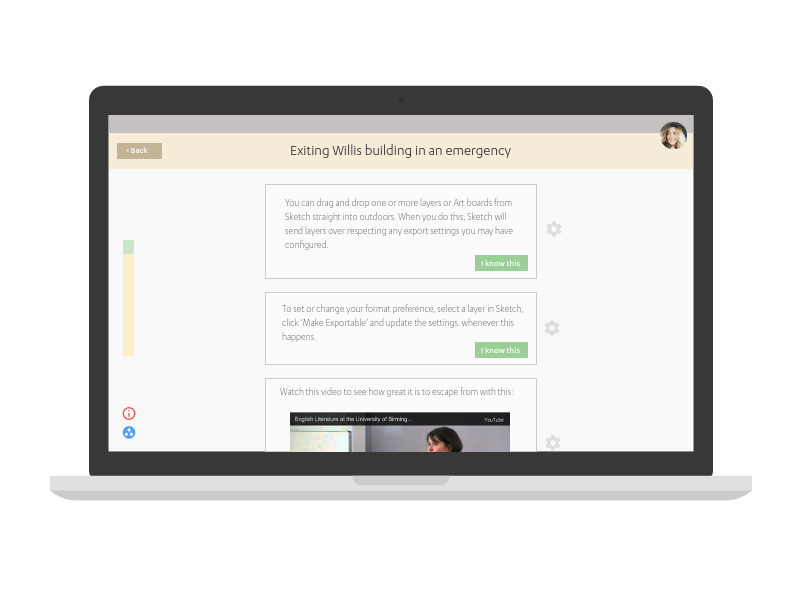
\includegraphics[width=\textwidth]{pitch-cards}
\caption{The initial pitch concept for the display of cards/facts}
\centering
\end{figure}
Tags associated with a decks allow for much more interaction with from the users and the decks. It would enable a user to ”subscribe” to certain tags, or a manager to decide what tagged decks are mandatory or recommended for an employee to complete and other similar actions.




%% $RCSfile: using.tex,v $
%% $Revision: 1.1 $
%% $Date: 2010/04/23 01:57:05 $
%% $Author: kevin $
%%
\chapter{Technology and Engineering Choices}

Before starting development on the product I needed to decide with HAUNT the best technologies and architecture to develop our product in. This includes the API architecture, any major JavaScript libraries that would have major implications in the development and any external services that we may want to implement such as external authentication.
This chapter will explore some of these options and explain any choices made and challenges that they may hold.
  
\section{API Architecture}
The first need is to provide an API service to access and modify database as required. The major decision that needed to be made was the choice between RESTful vs SOAP. Both are come with their pros and cons and are useful in different situations.

\subsection{SOAP}
SOAP is a web access protocol has long been the standard protocol when it comes to web services for its versatility. SOAP provides a way for application to communicate over a HTTP network. It is based on XML and is used to make requests and receive responses between an application and a service.
ADD SOME STUFF HERE
SOAP can quickly become complex and its architecture is more suited to operations and calls to action than simple database operations however it can do both. SOAP also supports multiple expansions to enhance its capabilities the major one being WS-Security which greatly increases security options and allows the use of various security token formats such as SAML (Security Assertion Markup Language). Because of this SOAP excels in many different environments but requires more customization and research into the required extensions. SOAP also has built in retry logic and error handling.

\subsection{REST - Representational State Transfer}
RESTful web services are a way of providing an application to to communicate with a service via a set of predefined stateless operations. RESTful services in general boast less bandwidth usage and faster response times \cite{mumbaikar2013web}

TODO
%%%TODO

\section{React - UI JavaScript Library}

React is a JavaScript library that is used to create interactive user interfaces easily. It was originally developed by engineers within Facebook when working on their own complex user interfaces. React brings a new concepts to web development, it shifts the generally accepted workflow of web development. React solves the problem of large scale user interfaces with data changes consistently \cite{reactintro2015}.

React allows you to `design simple view for each state in your application' and it will efficiently handle rendering the right components and automatically re-render the correct information and components when data changes\cite{react}. Traditionally the major problem when designing and developing a user interface is keeping it in sync with the business logic and state of the application and data \cite{staff2016react}.

\section{Summary}
\chapter{Agile and Lean Methodologies}

Software start up companies are required to be efficient with their development time and product analysis. There are two main methodologies that we will explore as possible solutions to implement during this development analysis at Haunt, Agile methodology and Lean methodology. Along with the overall methodology there are many tools and processes that you can utilize to implement the principles of your methodologies.

\section{Agile Methodology}
The Agile methodology was first created in February 2001 and is defined by the Agile Manifesto. It was designed specifically with software engineering in mind with the focus of the principles being customer satisfaction through early and continuous delivery of valuable software [1]. Agile methodology was developed for software development as the previous more rigid processes had expensive iteration cycles and did not fit the quickly evolving ideas and environment of software product development.

The principles in the Agile development are designed to produce a potentially shippable
product after each iteration, around 2-4 weeks depending on the implementation of which
process model. The principles from the Agile Manifesto:

\begin{itemize}
\item Satisfy the customer through early and continuous delivery of valuable software.
\item Welcome changes in requirements. Agile processes should be flexible.
\item Daily cooperation between business people and developers
\item The most efficient and effective method of conveying information to and within a development
team is face-to-face conversation.
\item Working software is the primary measure of success
\item Promote a sustainable development process and environment.
\item Continuous attention to technical excellence and good design enhances agility
\item Simplicity
\item Self-organizing teams
\item Regular reflection on how to become more effective and tune process appropriately.
\end{itemize}

Agile methodology is great for flexible development of the product that can adapt to
changing requirements and market environment.

\section{Lean Methodology}
Lean methodology is taken from the lean manufacturing process principles and translated into a software development environment. It originated in Toyota manufacturing around 1950 as Just-In-Time [4]. The main goals of lean methodology is to eliminate waste and work smarter not harder. Waste within a manufacturing context is easier to identify. Lean
manufacturing identified 7 main wastes. In a software development context these translated
into:
\begin{table}[h]
	\centering
	\begin {tabular}{|l|l|}
	\hline
	Toyota Manufacturing Wastes & Lean Software Development Wastes \\ \hline
	Inventory & Partially Done Work \\
	Extra Processing & Relearning \\
	Overproduction & Extra Features \\
	Transportation of Goods & Handoffs \\
	Waiting & Delays \\
	Motion (of people) & Task Switching \\
	Defects & Defects \\ \hline
	\end{tabular}
	\caption{Software Development Waste\cite{}}
\end{table}

To first eliminate these wastes you need to first identify some of their causes and follow a process that tries to minimise or eliminate them. These causes identified in Software Development Waste are very relevant in a startup company.
Building the wrong feature or product, creating features that no one needs or products that have little market are obviously not good investments of time and lead to waste (Extra Features).
Mismanagement of the backlog, focusing on features or products that offer worse value to the customer is obviously a less efficient use of development time and are often resulted in unfinished work when developers are needed to finish more important features (Partially done work).
Rework, if your software has a lot of defects/bugs or is not very robust or secure you will need to rework and refactor parts of it resulting in wasted time (Defects). Delays, in Lean Software Development delays refer to waiting for people to be available to provide required information.
Relearning refers to rediscovering something we knew [5]. And is either caused by forgotten decisions that have already been made or failing to communicate information effectively and therefor someone else rediscovering something that we already know.

\section{General Lean Process}
The generic process for Lean Software Development in a startup follows a Learn, Build, Measure process. Where you first gather information, gather required features and ideas, build a functional product that can be tested, test said product and gather data and then learn from that data and start the process again. Lean methodology and Agile methodology are closely related and Agile could be considered a subset of lean methodology that focuses on wasted time only. The key differences between agile and lean methodologies are that Lean focuses on reducing many types of waste to produce the product with the most value to the customer with little waste while agile more focused on constant integration and feedback to produce frequent iterations of the product that are always improving.

\begin{figure}[h]
\centering
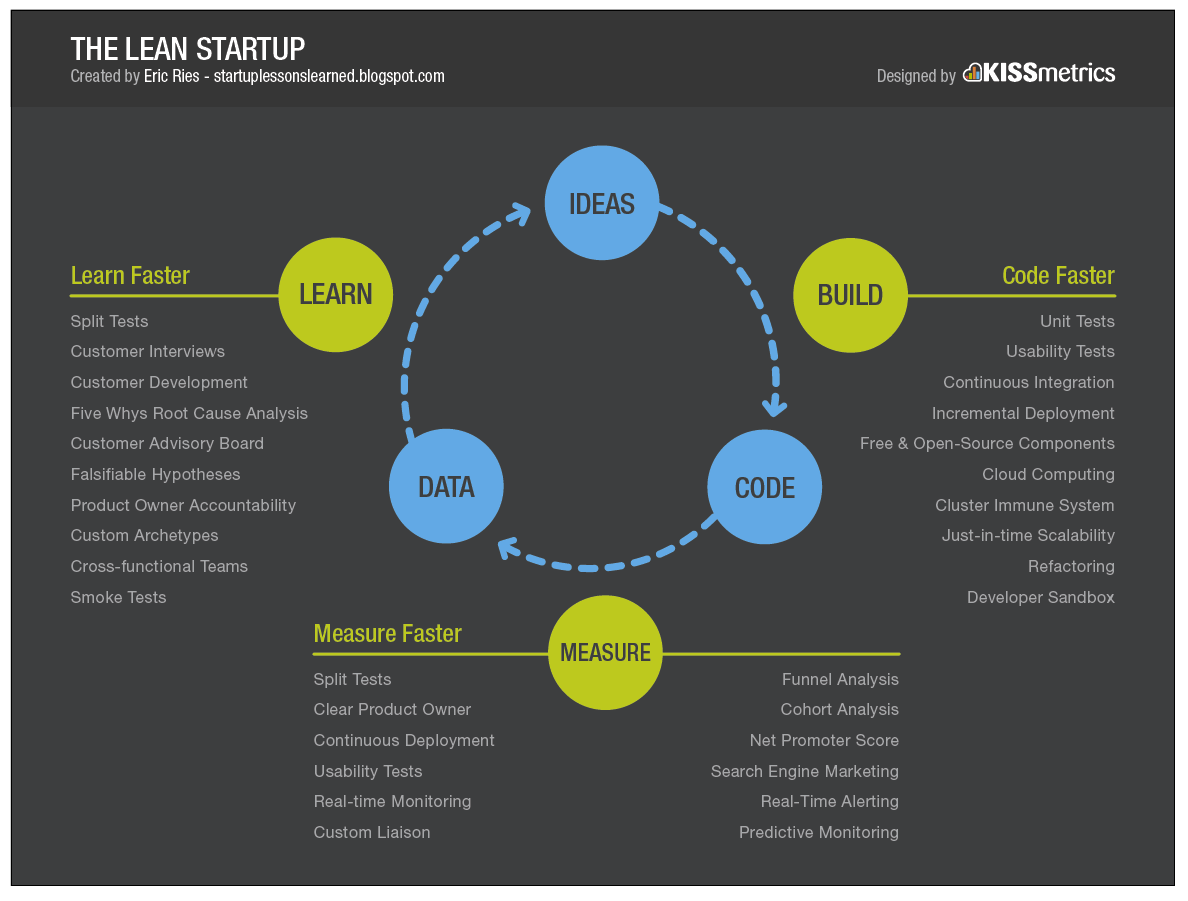
\includegraphics[height=7.5cm]{lean-flow}
\caption{Lean process model}
\end{figure}

\section{Process Models}

Both methodologies can utilize multiple process models that fit or can be adapted to adhere to their principles. Very common models are SCRUM for agile and KANBAN for lean.

\subsection{SCRUM}
SCRUM is an agile process model that focuses on having a potentially shippable product after each iteration called sprints. Each sprint normally lasts for around two weeks. The features or tasks that are worked on are taken from the backlog. The backlog is populated by user stories that have been collected from the client or product owner. They are use cases for potential features for the product

\begin{figure}[h]
\centering
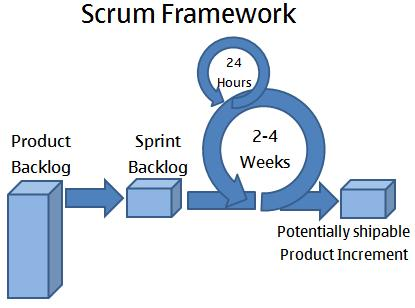
\includegraphics[height=4cm]{scrum-framework}
\caption{SCRUM process model}
\end{figure}

The SCRUM workflow begins with a planning stage for the sprint. The goal of the planning stage to to select and delegate the user stories to be completed this sprint. During this planning stage you select and evaluate the difficulty of user stories to be completed during the coming sprint. Then the daily scrum is used to say what each team member will work in the next 24 hours to achieve this goal. This is repeated until the end of the sprint. After a sprint you would have a potentially shippable product and there is a review and reflection process as well.

\subsection{Extreme Programming: XP}

Extreme programming (XP) was one of the first agile methodologies. It was designed to solve the problems of heavier, more formal methodologies and be more flexible and efficient as explained by Kent Beck, XP is a lightweight methodology for small-to-medium-sized teams developing software in the face of vague or rapidly changing requirements. [2]. XP is similar to scrum in the fact that it emphasizes frequent releases and shorter development cycles. Along with advocating pair programming, code review and unit testing on all code. The basic principles of XP are [2]:
\begin{itemize}
\item Rapid feedback
\item Assume simplicity
\item Incremental change
\item Embracing change
\item Quality work
\end{itemize}

\begin{figure}[h]
\centering

\includegraphics[height=7cm]{xp-flow}
\caption{XP process model}
\end{figure}

XP is highly flexible and can easily manage in an environment of rapidly changing requirements. It is simple and easily understood and can be implemented with any team that is familiar with agile methods and manifesto. It relies heavily on pair programming and automated unit testing.

\chapter{Implementation}
For the implementation of this project we decided to implement a agile methodology approach similar to other projects run at  Haunt. The main process model that we will be taking much of the development process from are aspects of SCRUM. The development was split into multiple sprints, with each containing a requirements gathering stage, development and reflection stage. Each sprint will start with a client meeting with Haunt where we will populate the backlog and develop user stories as requirement gathering. Later on in the development we planned to include meetings with potential users and experts for feedback on the implemented solutions and gather more insight for more efficient user stories. However due to unforeseen circumstances we were only able to gather expert feedback within the final sprint. One of the key features of lean and agile methodology is saving on waste. To try and implement this we will focus on building the core product/prototype first and then gain feedback on the product via user testing to gather more specific features and requirements for the product.

\section{Initial Product}
At the start of the project Haunt had a preliminary proof of concept that needed to be further developed. This initial product contained an API that could add cards, decks and users. The front end consisted a simple view that could display the contents of the decks and cards related to the user. The API was developed in Ruby and followed the RESTful architecture, with the front end developed in JavaScript with Redux js for front end state control. All authorization was done through Auth0 as a temporary solution.

\section{Pre-Development}
Before initial development started we first needed to establish what aspect of the product we would be focusing on. Initially the plan was to develop a potential dashboard for the product. However because development on the main product prototype was no longer in progress via Haunt, this project changed focus to general development of the product.
During the first meetings with the product owner, Rob McGrail, Technical Director at Haunt, we established that some of the underlying technologies on both the front end and api side were either excessive or not long term solutions and needed to be removed. These were identified as state control via redux and the authentication system through Auth0, the first sprint was focused on removing these required technologies to reduce future development time. The later sprints would be focused on refining, adding and fleshing out features in the product.

\section{Sprint 1}
As stated above the first sprint was focused on reducing the overhead of future development by removing unnecessary and excessive factors of the  initial proof of concept, namely the authorization system Auth0 and the front end state management control redux js. The product owner and I deemed this an important step to reduce waste at later stages of development and not build up technical overhead.

\subsection{Auth0}
Auth0 is a third party single sign on and token based authentication system that the initial proof of concept was using for user authentication. While this was easy to setup and manage, it was not a suitable long term solution due to extra costs incurred through licensing and extra latency of  relying on a third party service instead of having the authentication handled by the same service as the Restful API. Auth0 would potentially be able to provide better security of data and more complex 
After some consideration we decided it was best to replace the authentication with a JSON web token (JWT) system as it is industry standard for `URL-safe means of representing claims to be transferred between two parties'\cite{jones2015rfc}.

\subsection{JWT Tokens}
JSON web tokens consist of an encrypted token that contains a payload consisting of a JSON object and is encrypted via a JSON web signature. Using these JWT tokens we are able to securely authenticate users and produce a token for them that tells the API their user role, organisation, id and creation date. This allows them to stay logged in securely and helps govern access to the API based on their role.

\subsection{Redux JS}
Redux is a state container for JavaScript applications, it was used to keep the current state of the front end under control to help lower load times and preserve data and scope. Redux is a great tool for managing your app state in a way that allows states to persist through the same session or even through sessions if saved locally. However it comes with some trade offs and requires you to structure your apps data in certain ways:

\begin{itemize}
\item State needs to be described as plain JSON objects and arrays.
\item Describe changes in the system as plain objects
\item Any logic for handling changes to the state needs to be as pure functions
\end{itemize}

These requirements for how you structure logic, state and changes within the system make sense and are often good practices to follow if you wish for your code to be decouple what happened, for example a button press or data finish loading with how this changes things, for example when the data is loaded change the values on screen. However because of the relatively simple states required for this web application and no foreseeable need for a persistent state. It was decided that maintaining the state store through Redux was not required and the app.

So for this sprint the main focus was removing these unnecessary libraries and replace them with current solutions. The Auth0 authentication service was replaced with our own JWT focused authentication using and redux state management was replaced with logic within the components.

\subsection{Summary}
With this sprint focused on removing some of the system that were no longer required a lot of this sprint went into refactoring the code base and implementing the new authentication system. The refactoring of removing redux from the system included moving the action logic for components into the components themselves. This reduced the indirection within the code but more tightly couples the components with the logic and actions of the system. This means that it is harder to implement another component with very similar features that should act the same way but with a different look or display. This was considered a reasonable trade off as it simplifies the workflow of each action and makes the code easier to follow, because the products logic flow should be reasonably simple with no overly complex actions or components.


 \begin{figure}
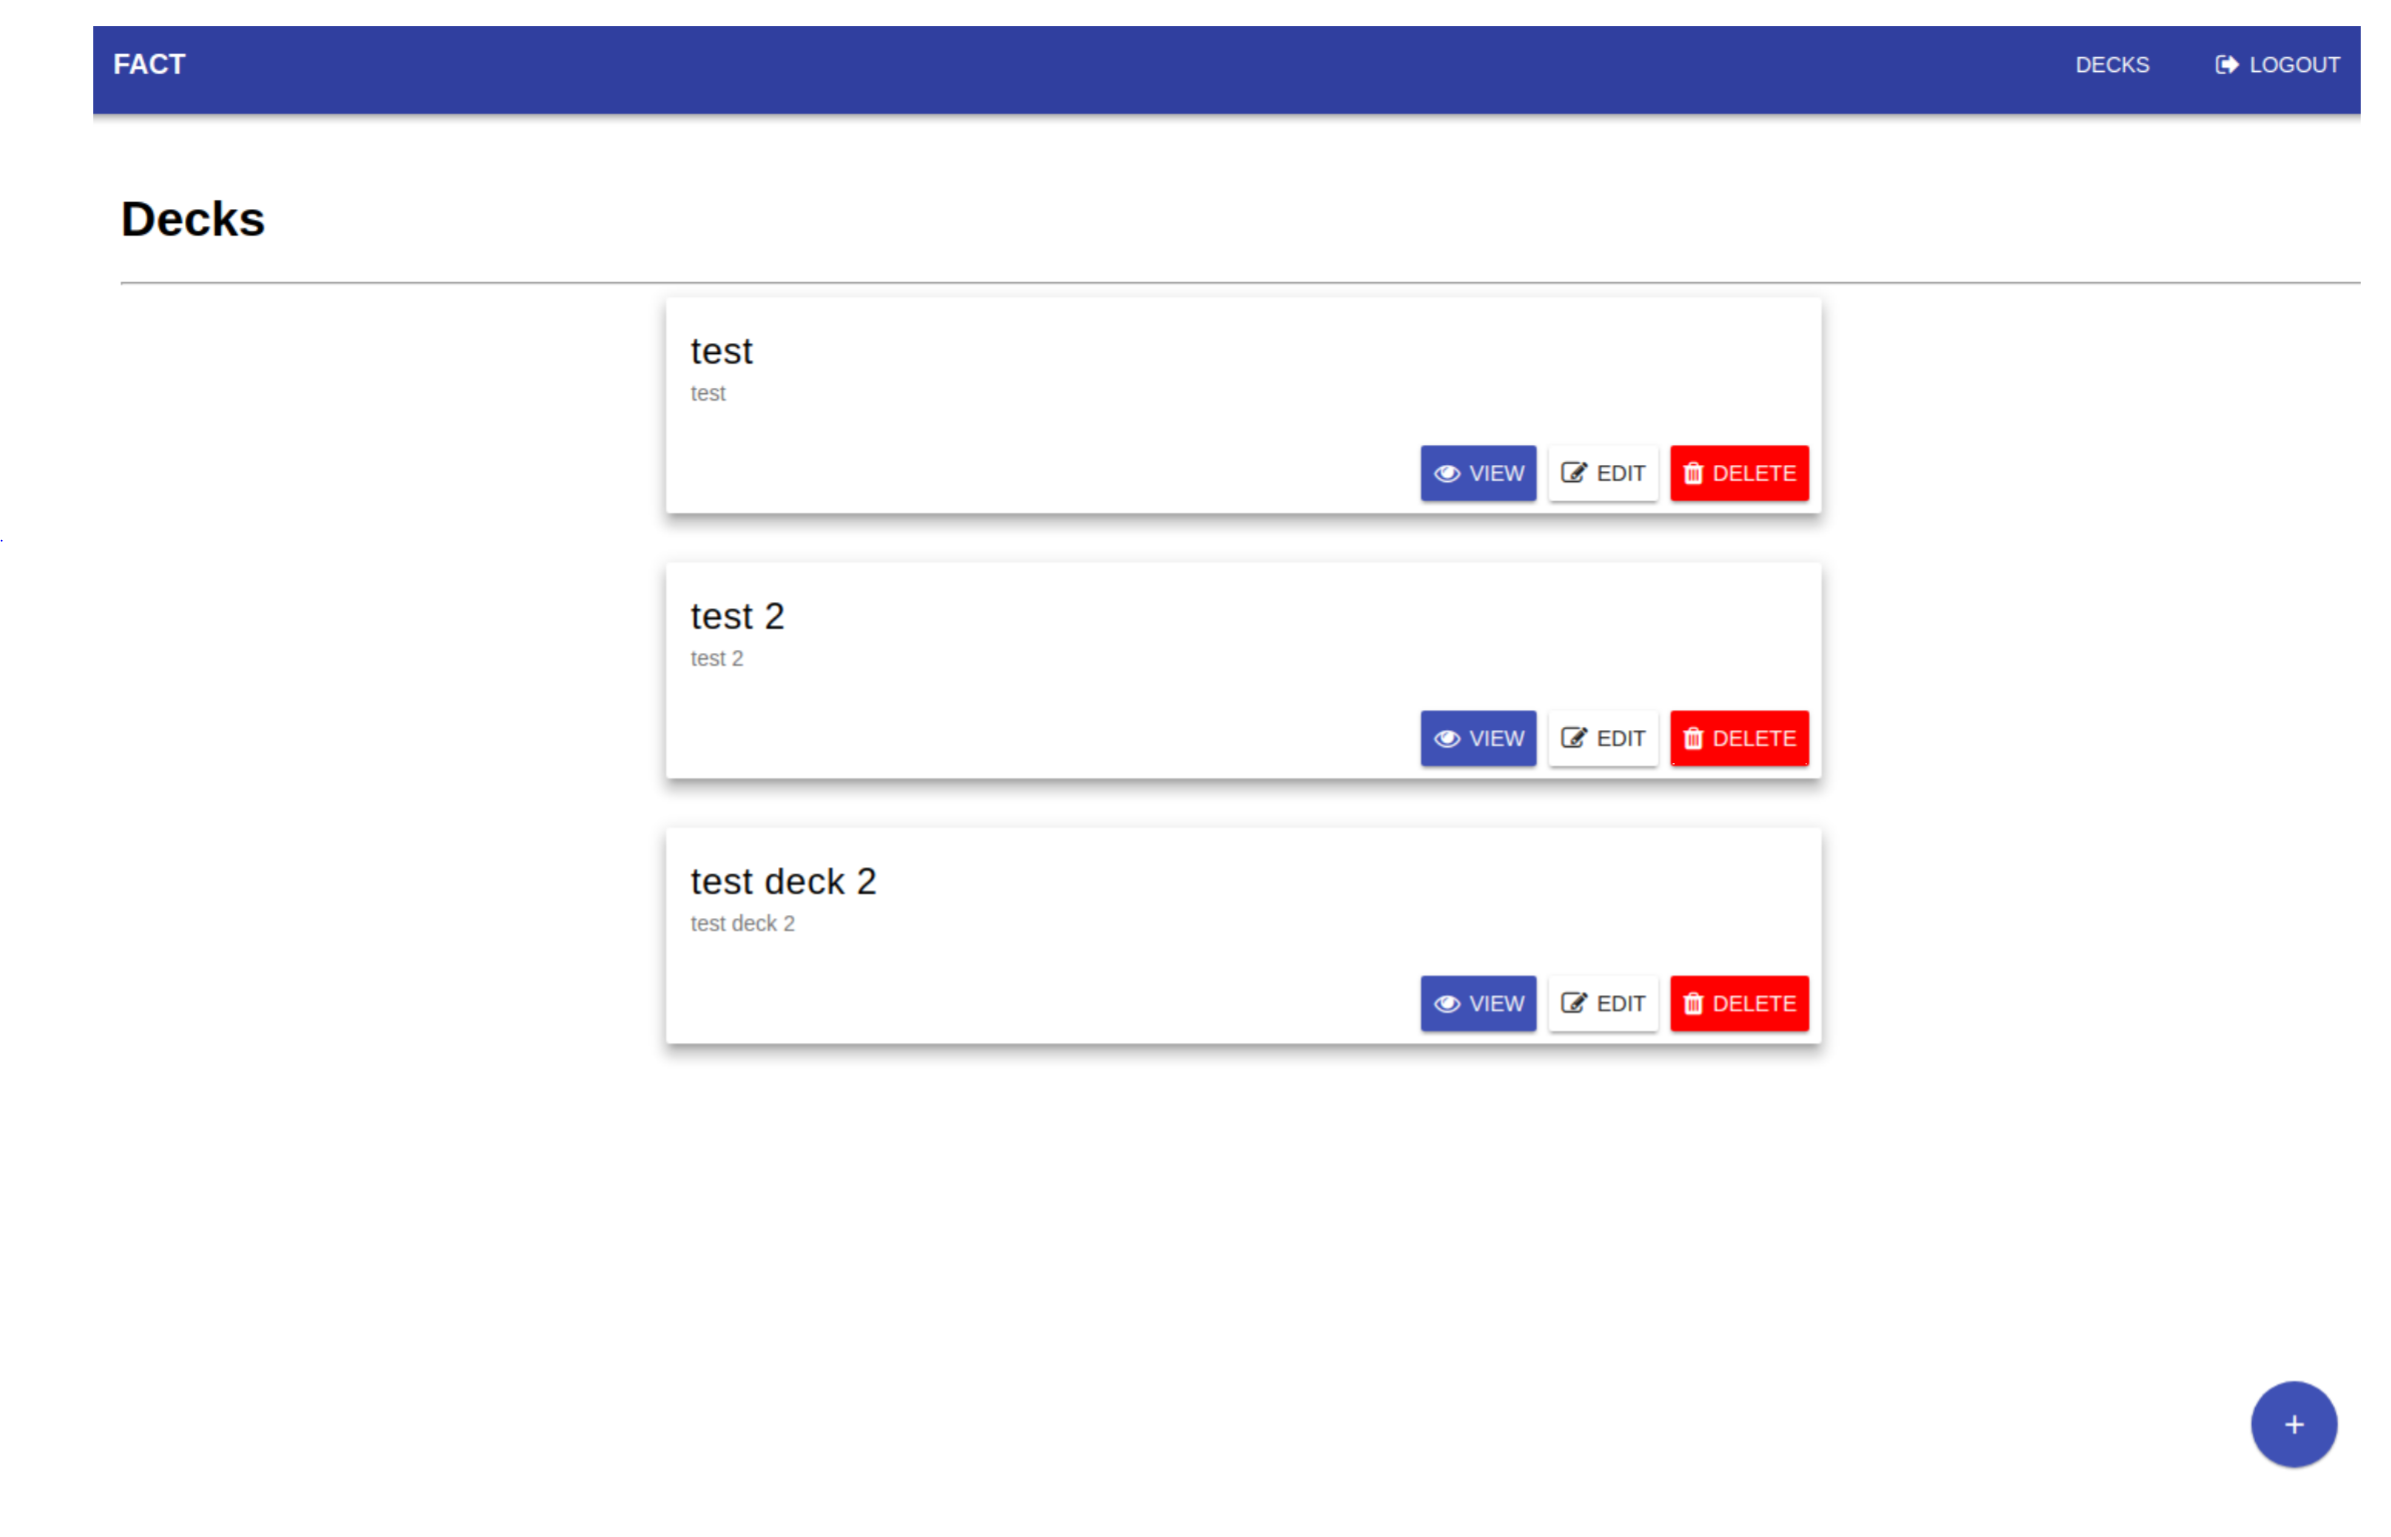
\includegraphics[width=\textwidth]{s1}
\caption{Display of a fact deck after development in sprint 1}
\centering
\end{figure}

\section{Sprint 2}
This sprint was targeted towards getting some of the key features functional and in a state where the app could be used functionally. The initial proof of concept had some of the features like deck and card creation, user and organisation creation and the ability to view decks/cards linked to your organisation. The next major step was getting editing for all of the assets and tidying up the interfaces for managing the decks and cards.

\subsection{Improving Workflow of Cards and Decks}
One of the major problems identified with the work flow of the proof of concept was the disconnect between the list view and the creation of cards and decks. Initially creating a new card would bring up a separate screen with a separate url. This disconnects the content from the context of the deck or organisation. To improve the user experience when creating cards and decks, I implemented an inline feature for adding cards. To do this I changed the creation form to be displayed as a card the same as the current cards within the deck. This made it so when you start adding a card it will display it in the list and allow you to fill out the details within the card without changing changing page or view. 

 \begin{figure}
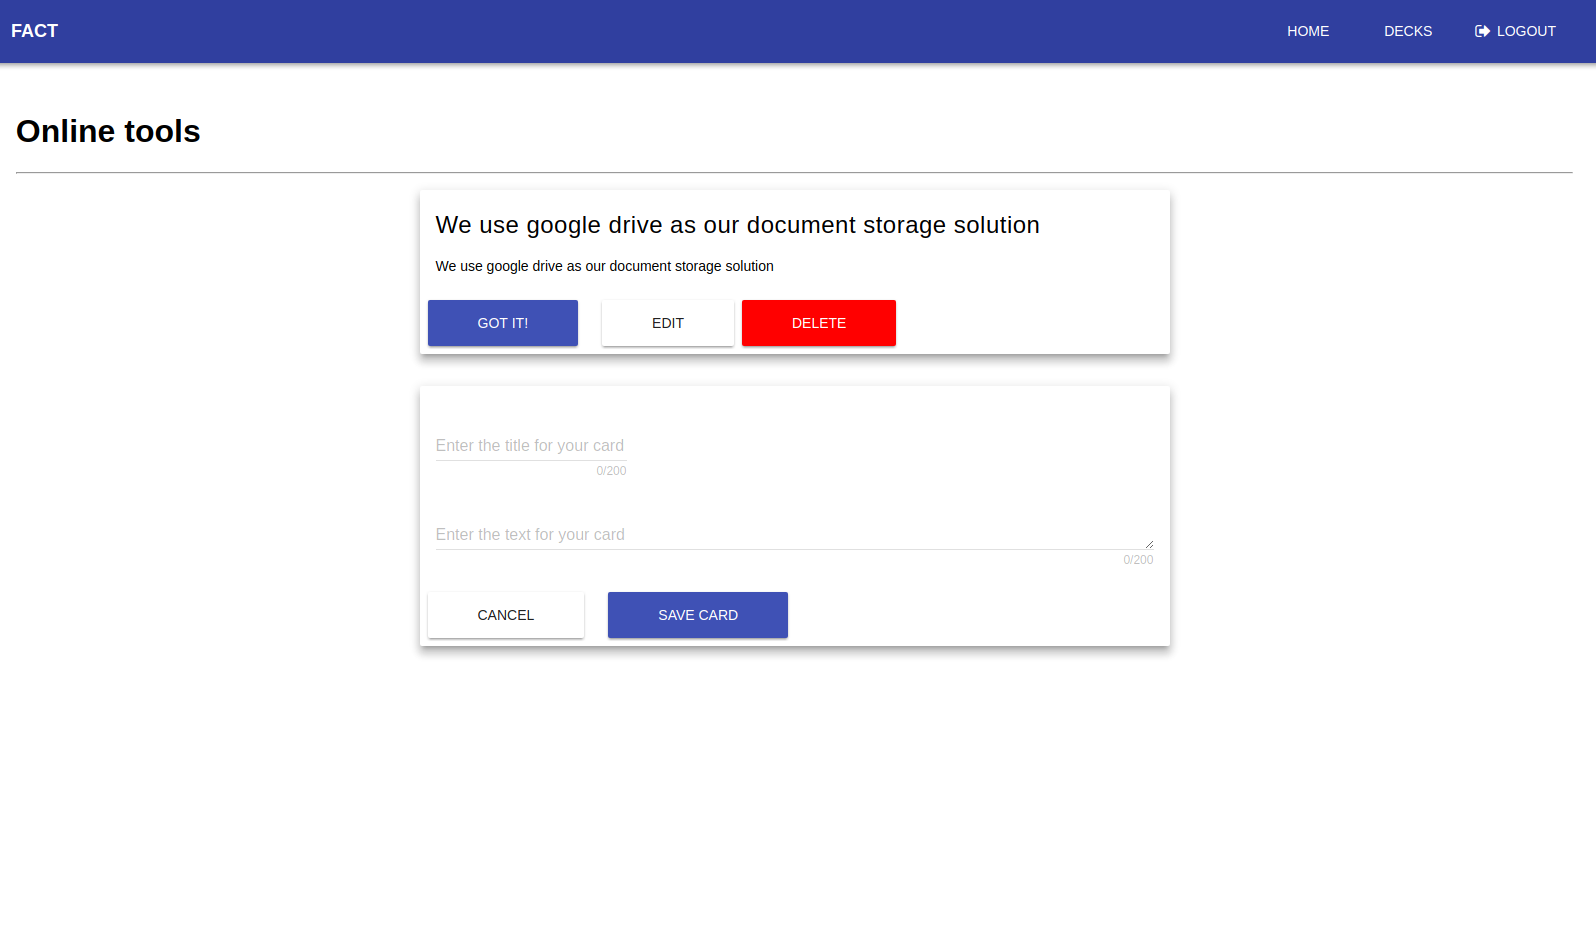
\includegraphics[width=\textwidth]{s2-edit-2}
\caption{Card creation after sprint 2}
\centering
\end{figure}


This change streamlined the user experience and made it more clear what the creation of cards and deck was doing and the general structure of the information. This in display creation and editing can be seen in many other web applications that use a card based display system such as Trello and Basecamp (see appendix: \ref{appendix:cardResearch}).

\subsection{Cards and Deck Editing}
During this sprint I added editing to the cards for both decks and cards this used the same system as the card creation just with different actions. This allowed me to reuse the same react component with different actions passed to it. This highlights the uses for react and the flexibility it brings when it comes to code reuse.

\subsection{Summary}
At the end of this sprint we went through the basic features that we needed to implement for a minimum viable product and identified some of the major ones that the product was still missing. It was also discussed about changing the component library we were currently using as it had limited design space and the overall default styling was not close enough to the final goal for the minimum viable product.
\section{Sprint 3}

\begin{itemize}
\item Added tags to decks
\item Finished api database shema allowing for more info in cards, including title and limit characters and card completions
\end{itemize}

 \begin{figure}
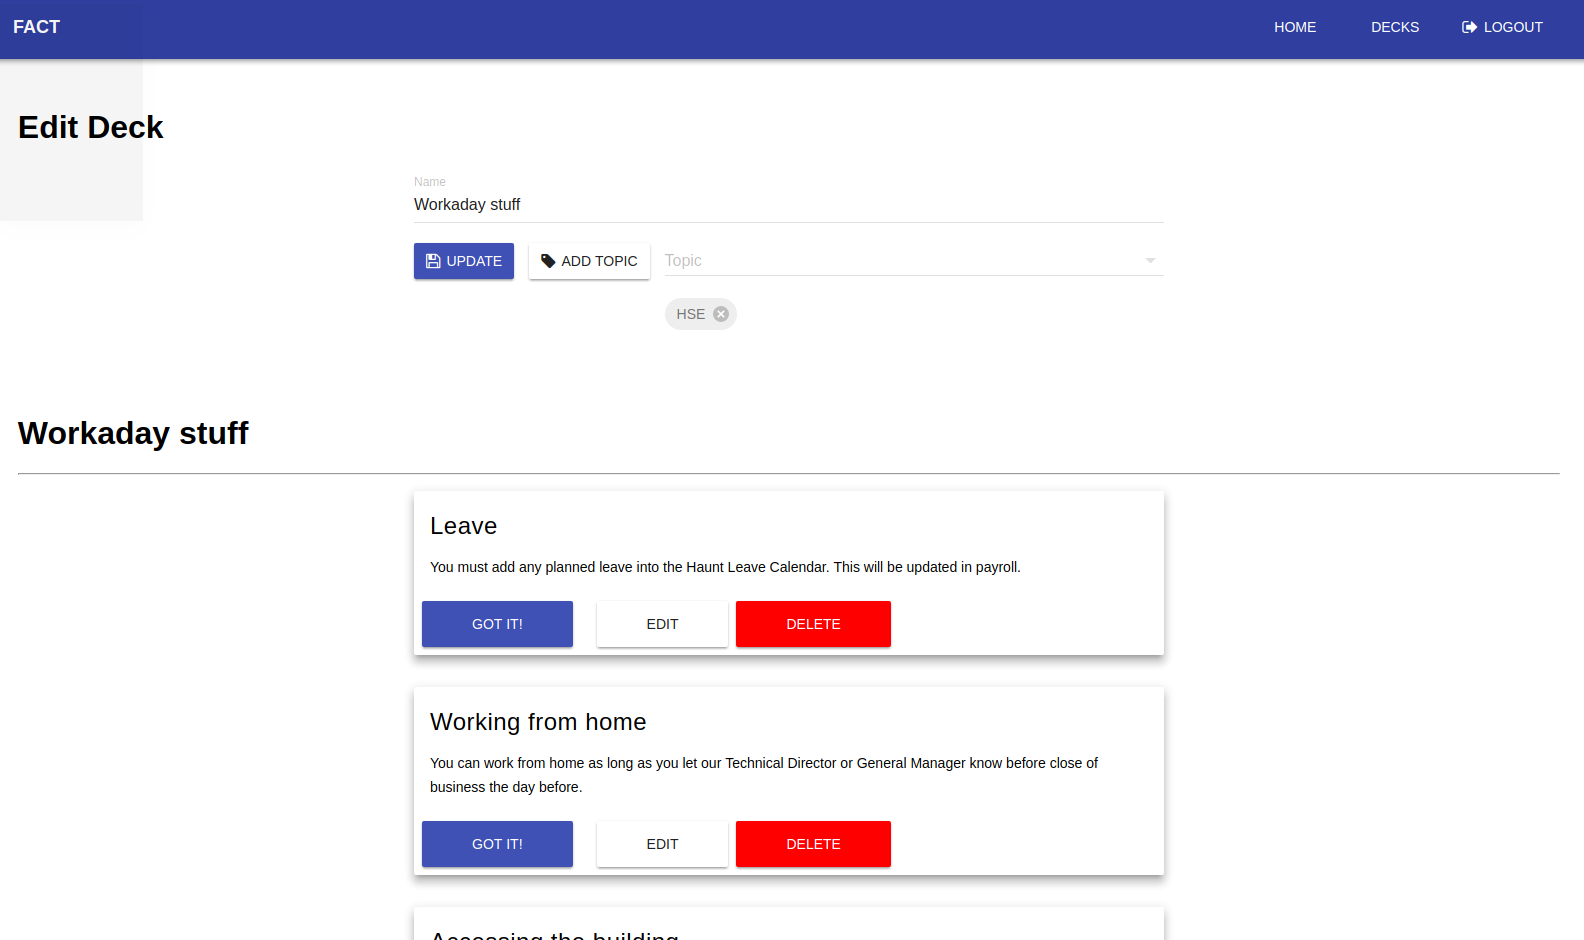
\includegraphics[width=\textwidth]{s3-tags}
\caption{The inclusion of tags in sprint 3}
\centering
\end{figure}

\section{Sprint 4}
This sprint was the final sprint

\begin{itemize}
\item Added
\item completion bar
\item new layout
\item create buttons
\item drop down actions
\item links in cards
\end{itemize}

 \begin{figure}
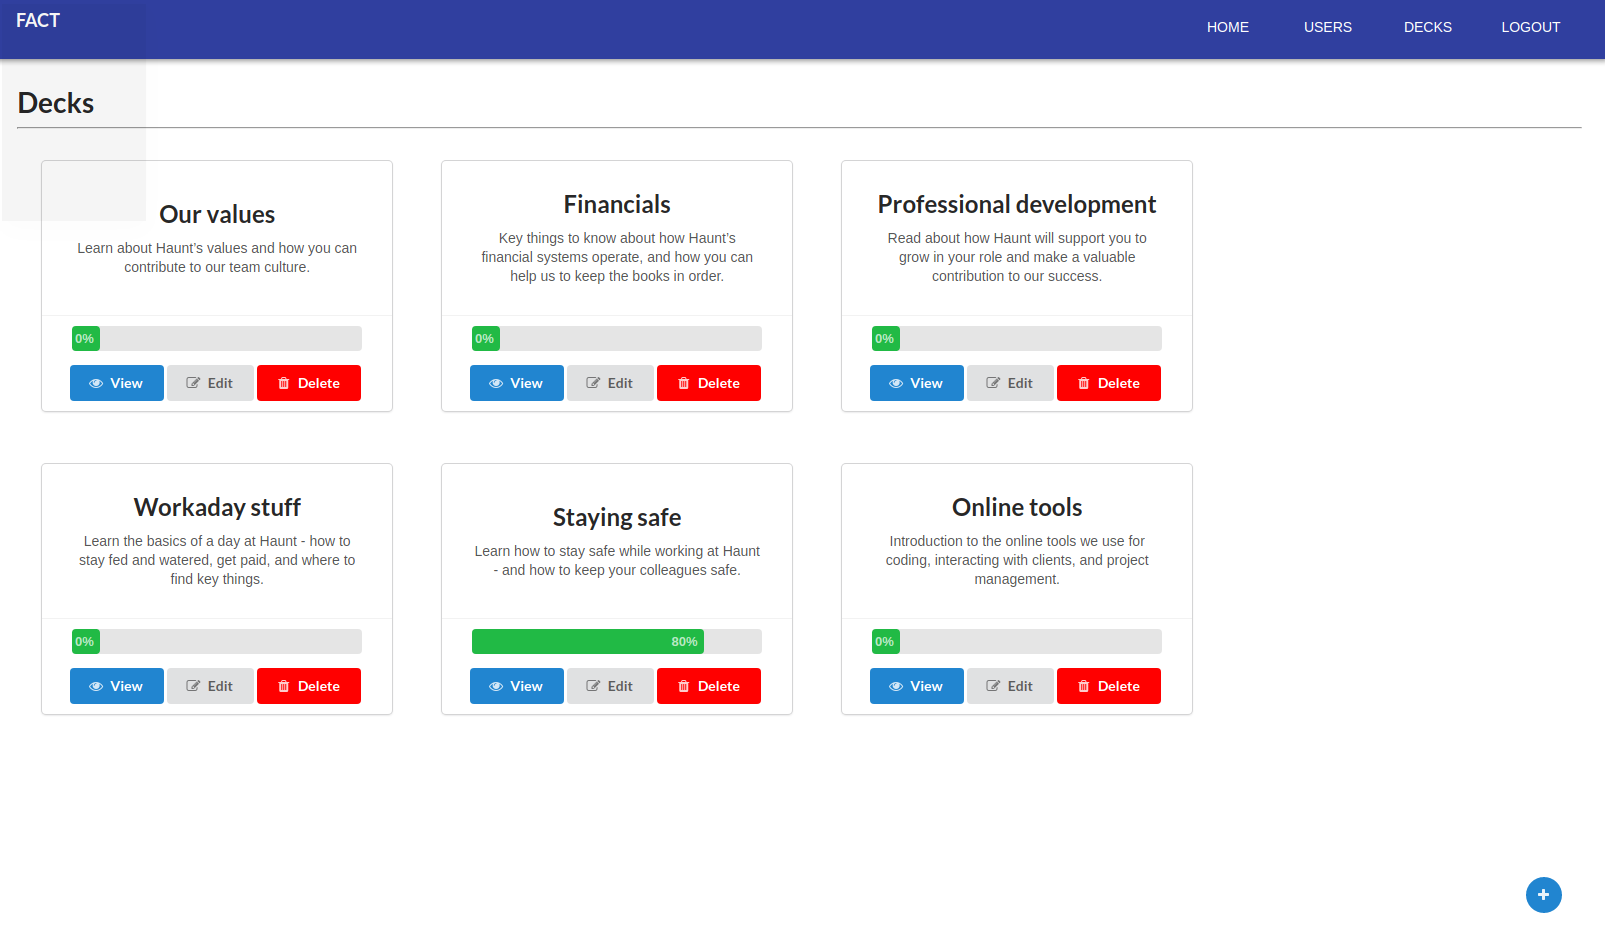
\includegraphics[width=\textwidth]{s4-decks}
\caption{Deck display after final sprint}
\centering
\end{figure}

 \begin{figure}
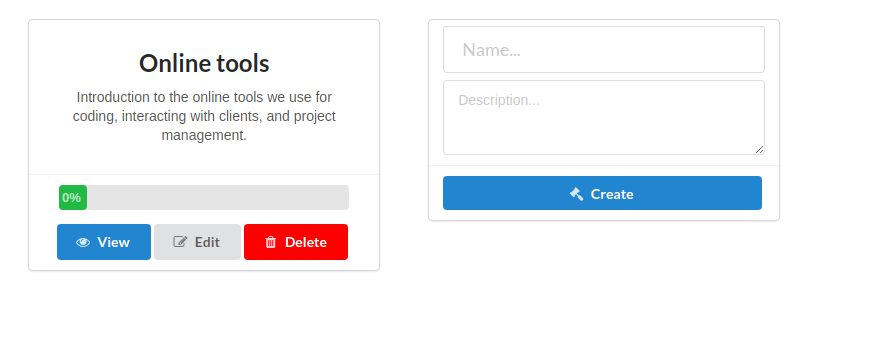
\includegraphics[width=\textwidth]{s4-deck-add-2}
\caption{Deck creation interface after final sprint}
\centering
\end{figure}

 \begin{figure}
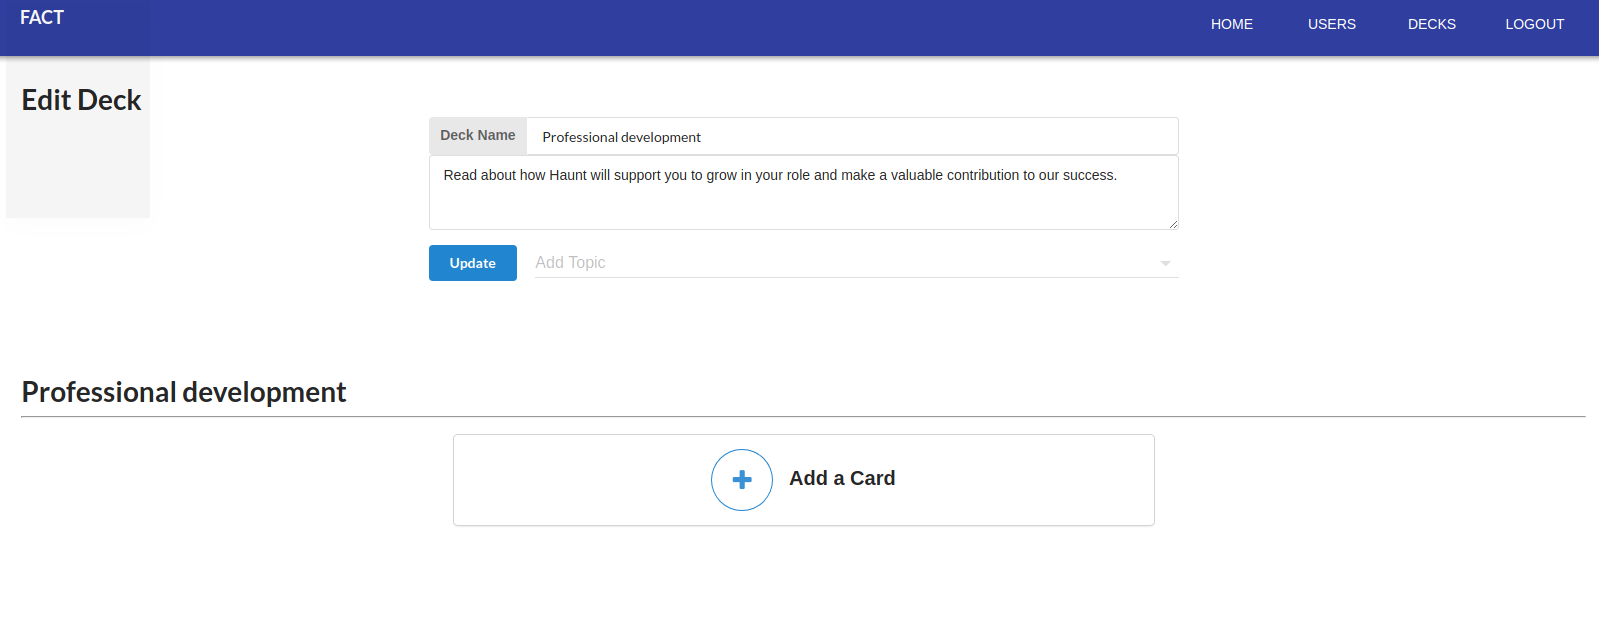
\includegraphics[width=\textwidth]{s4-deck-edit}
\caption{Deck edit interface after final sprint}
\centering
\end{figure}


 \begin{figure}
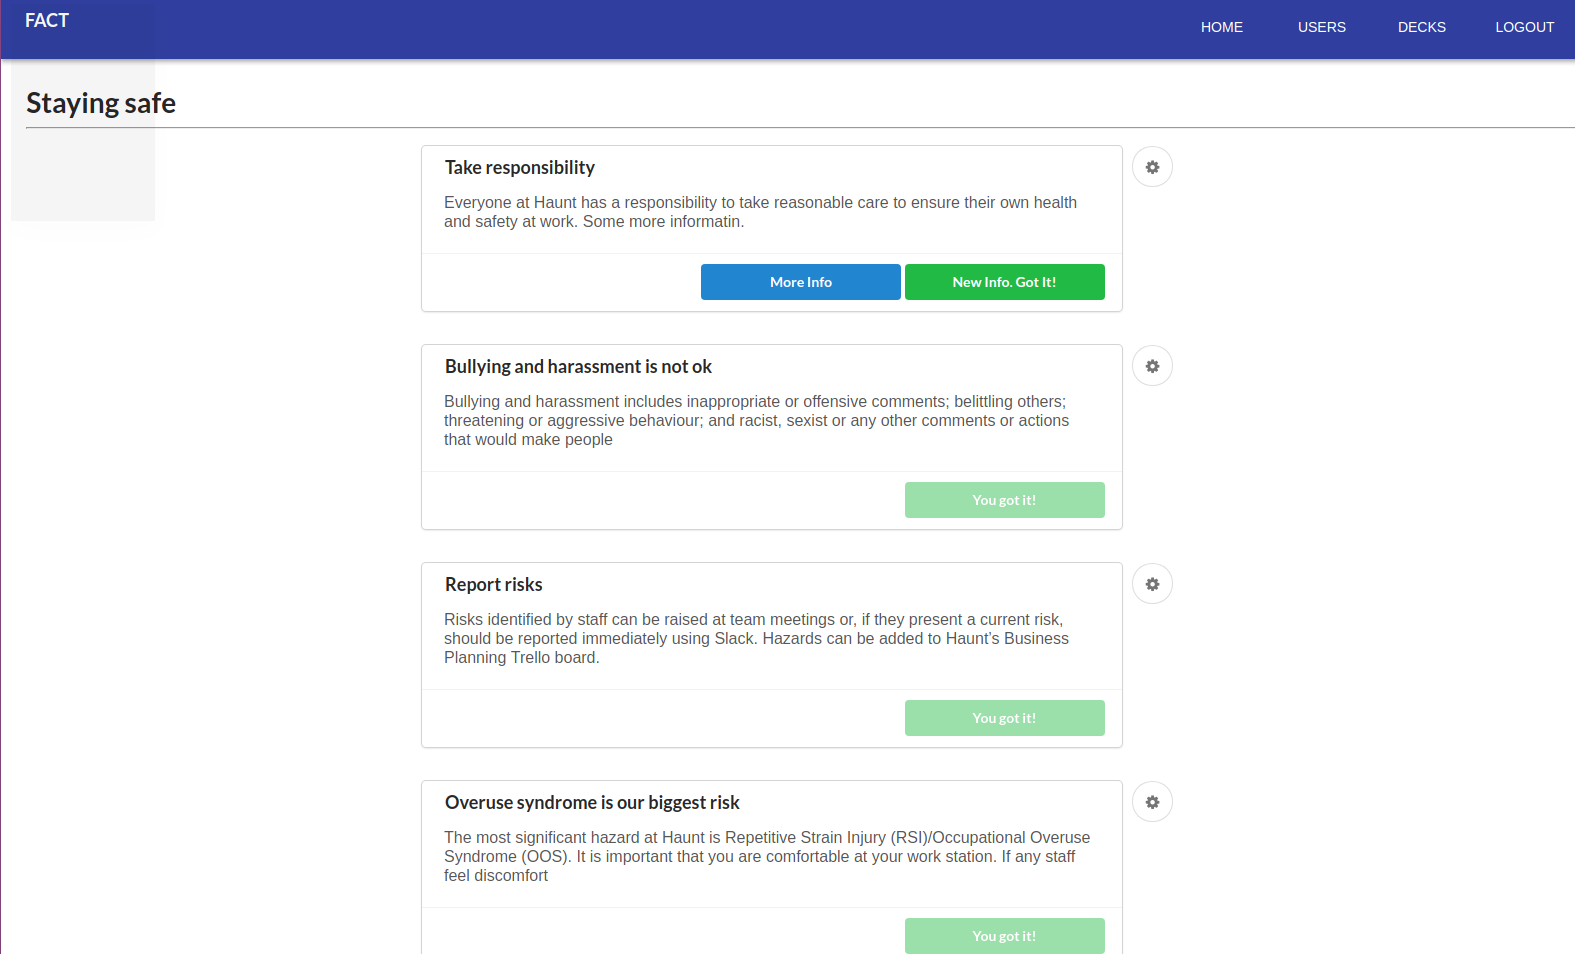
\includegraphics[width=\textwidth]{s4-cards}
\caption{Cards display after final sprint after final sprint}
\centering
\end{figure}

 \begin{figure}
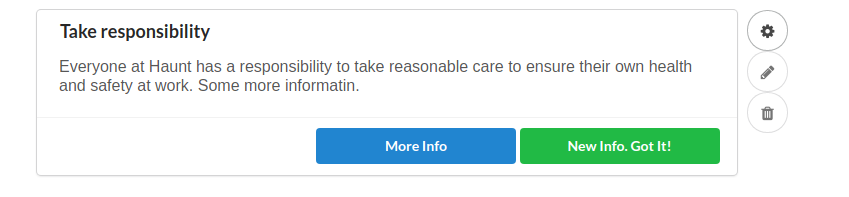
\includegraphics[width=\textwidth]{s4-card-actions}
\caption{Card action dropdown after final sprint}
\centering
\end{figure}

 \begin{figure}
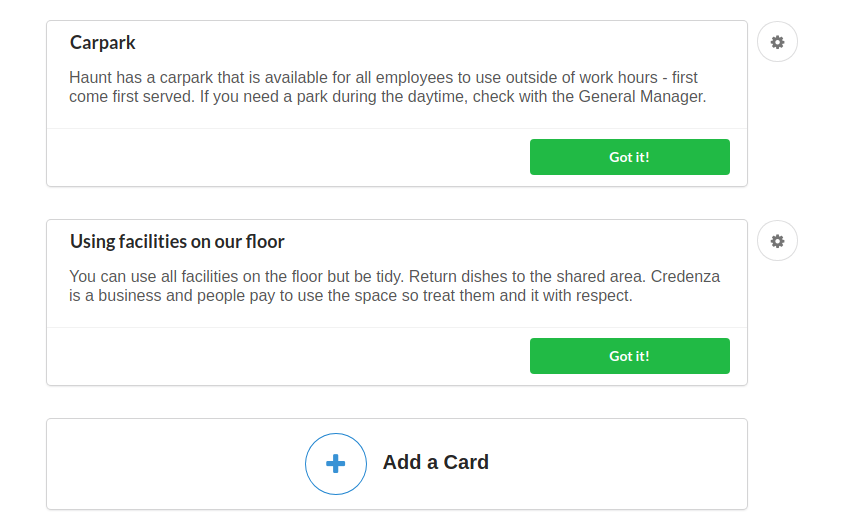
\includegraphics[width=\textwidth]{s4-card-add}
\caption{Card adding interface after final sprint}
\centering
\end{figure}

 \begin{figure}
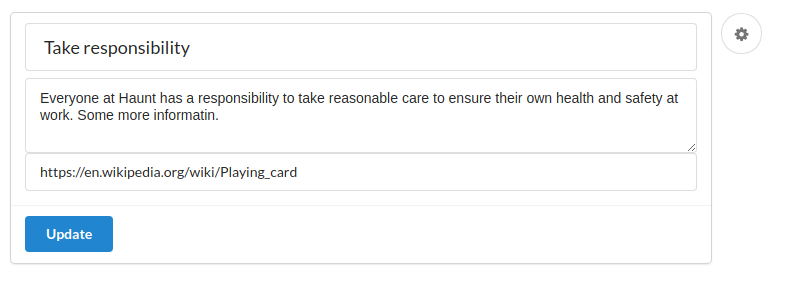
\includegraphics[width=\textwidth]{s4-card-edit}
\caption{Card adding interface after final sprint}
\centering
\end{figure}


\chapter{Industry and Expert Feedback}
\chapter{Comparrison to current solutions}
\chapter{Conclusions}\label{C:con}
The conclusions are presented in this Chapter.



%%%%%%%%%%%%%%%%%%%%%%%%%%%%%%%%%%%%%%%%%%%%%%%%%%%%%%%

\backmatter

%%%%%%%%%%%%%%%%%%%%%%%%%%%%%%%%%%%%%%%%%%%%%%%%%%%%%%%


%\bibliographystyle{ieeetr}
\bibliographystyle{acm}
\bibliography{sample}

\begin{appendices}
\chapter{Card Research}
\label{appendix:cardResearch}
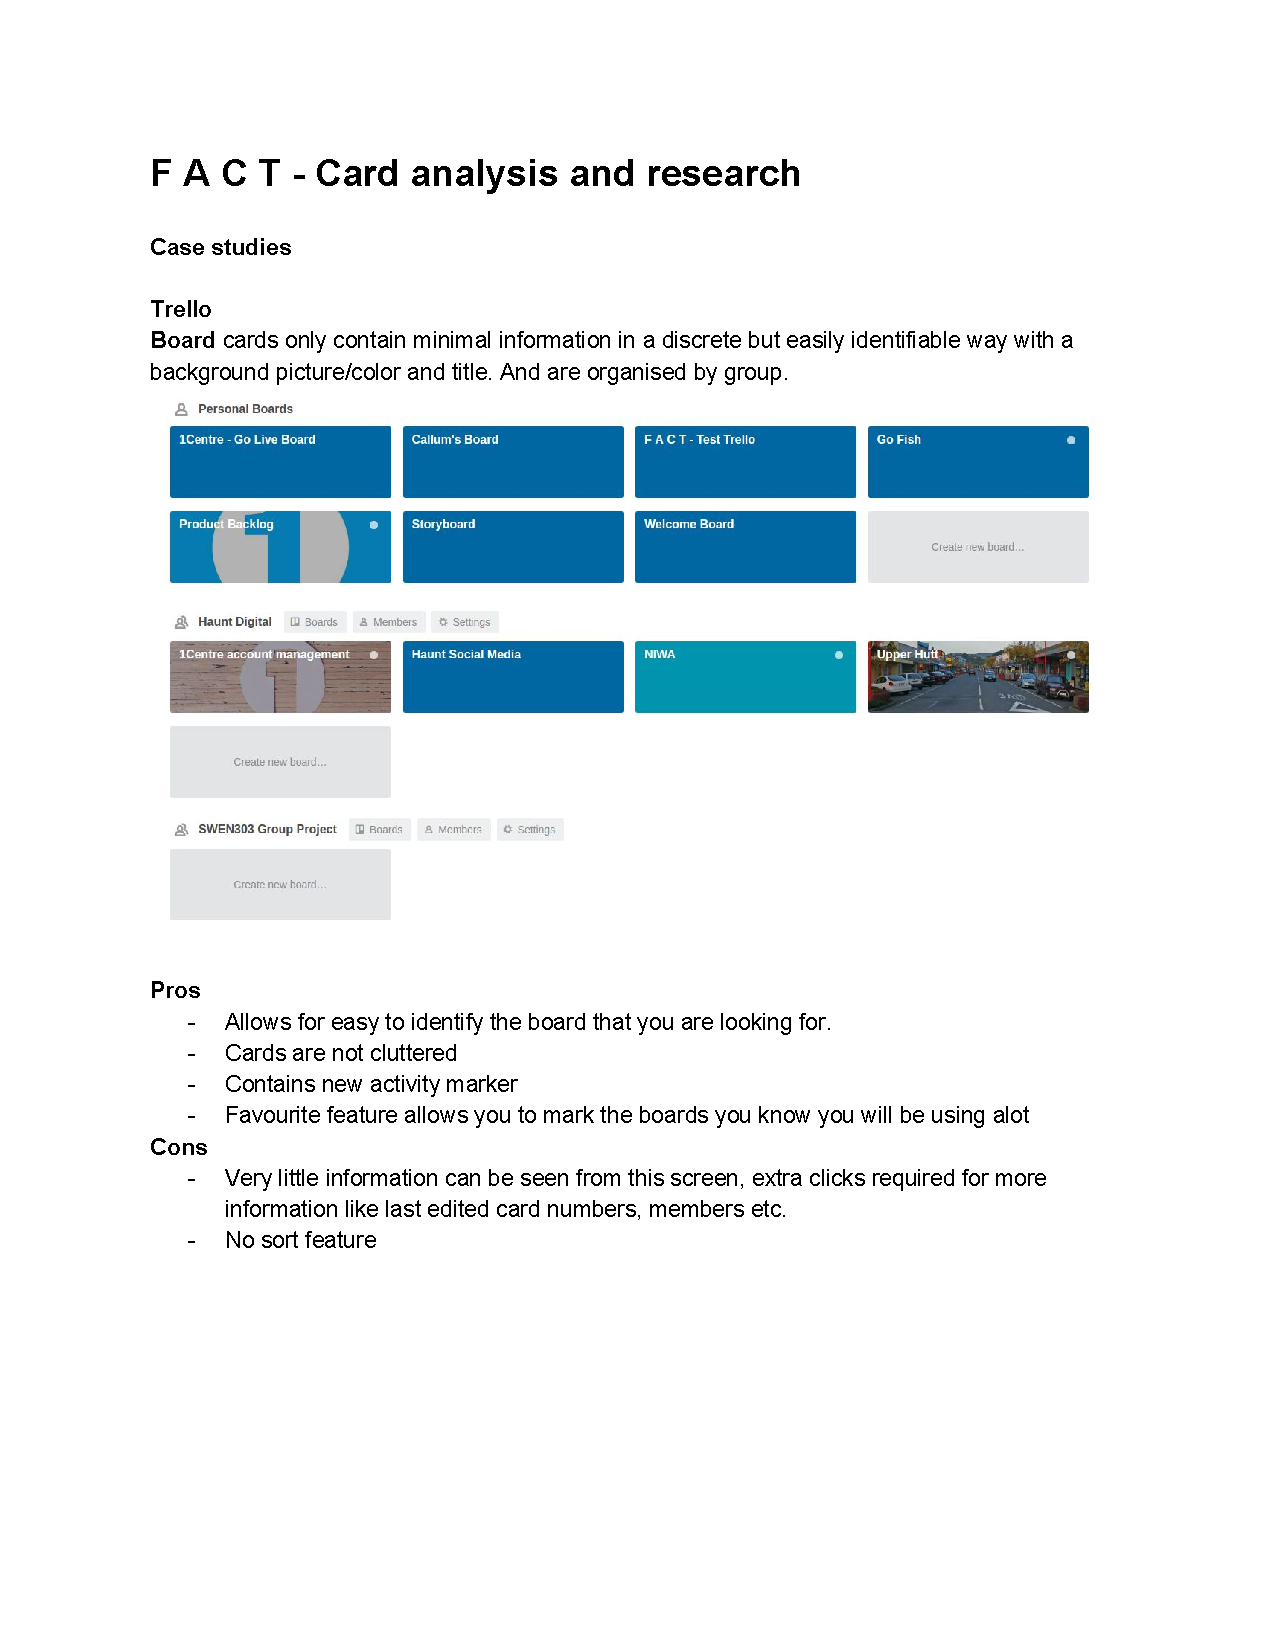
\includegraphics[page=1,scale=0.8]{cardResearch.pdf}
\includepdf[pages={2-},scale=0.8]{cardResearch}
\end{appendices}


\end{document}
